% Homework Requirements
% - What are the motivations for this work?
% - What is the proposed solution?
% - What is the work’s evaluation of the proposed solution?
% - What is your analysis of the identified problem, idea, and evaluation?
% - What are future directions for this research?
% - What questions are you left with?

\documentclass[12pt]{article}

% Font family
\usepackage{xeCJK}
\setCJKmainfont{Noto Serif TC}
\usepackage{amssymb}
\usepackage{amsmath}

% Document layout
\usepackage[margin=2cm, a4paper]{geometry}
\usepackage{setspace}
\onehalfspacing
\setlength{\parskip}{12pt}
\setlength{\parindent}{0pt}

% Citation
\usepackage{biblatex}
\addbibresource{./ref.bib}

% Image
\usepackage{graphicx}
\graphicspath{{./images/}}

% \title{Paper Review Assignment 1}
% \author{施宇庭}

\begin{document}
% \maketitle

%%%%%%%%%%%%%%%%%%%%%%%%%%%%%%%%%%%%%%%%%%%%%%%%%%%%%%%%%%%%

\begin{titlepage}
\begin{center}

\vspace*{1cm}
\large EAI 2024 Fall \\
\Large Paper Review Assignment 2 \\

\vspace{2cm}
\LARGE \textbf{A Review of "Deep Compression: Compressing Deep Neural Networks with Pruning, Trained Quantization and Huffman Coding"} \\

\vfill
\normalsize
學生:施宇庭 NN6124030 \\ [0.2cm]
指導教授:蔡家齊 \ 助理教授 \\ [0.2cm]

\end{center}
\end{titlepage}

% \pagebreak \tableofcontents \pagebreak

%%%%%%%%%%%%%%%%%%%%%%%%%%%%%%%%%%%%%%%%%%%%%%%%%%%%%%%%%%%%

\section{Motivation}

The goal of this paper is to compress deep neural networks (DNNs) required to run inference with large models on edge/mobile devices. The motivation for this work is to address the following challenges:

\begin{itemize}
    \item Reduce model size
    \item Reduce memory footprint
    \item Improve inference speed
    \item Reduce communication overhead
    \item Reduce energy consumption
    \item Maintain model accuracy
\end{itemize}

With the insight that pruning and quantization are able to compress the network without interfering each other, They proposed "Deep Compression" combining pruning, quantization, and Huffman coding to keep accessing weights on chip instead of going to off-chip DRAM.

%%%%%%%%%%%%%%%%%%%%%%%%%%%%%%%%%%%%%%%%%%%%%%%%%%%%%%%%%%%%

\section{Proposed Solution}

This paper proposes the "Deep Compression" method, which combines pruning, quantization, and Huffman coding to compress neural networks to 1/35 to 1/49 of their original size while maintaining the same accuracy as the uncompressed network, as illustrated in Figure \ref{fig:method_overview}.

\begin{figure}
    \centering
    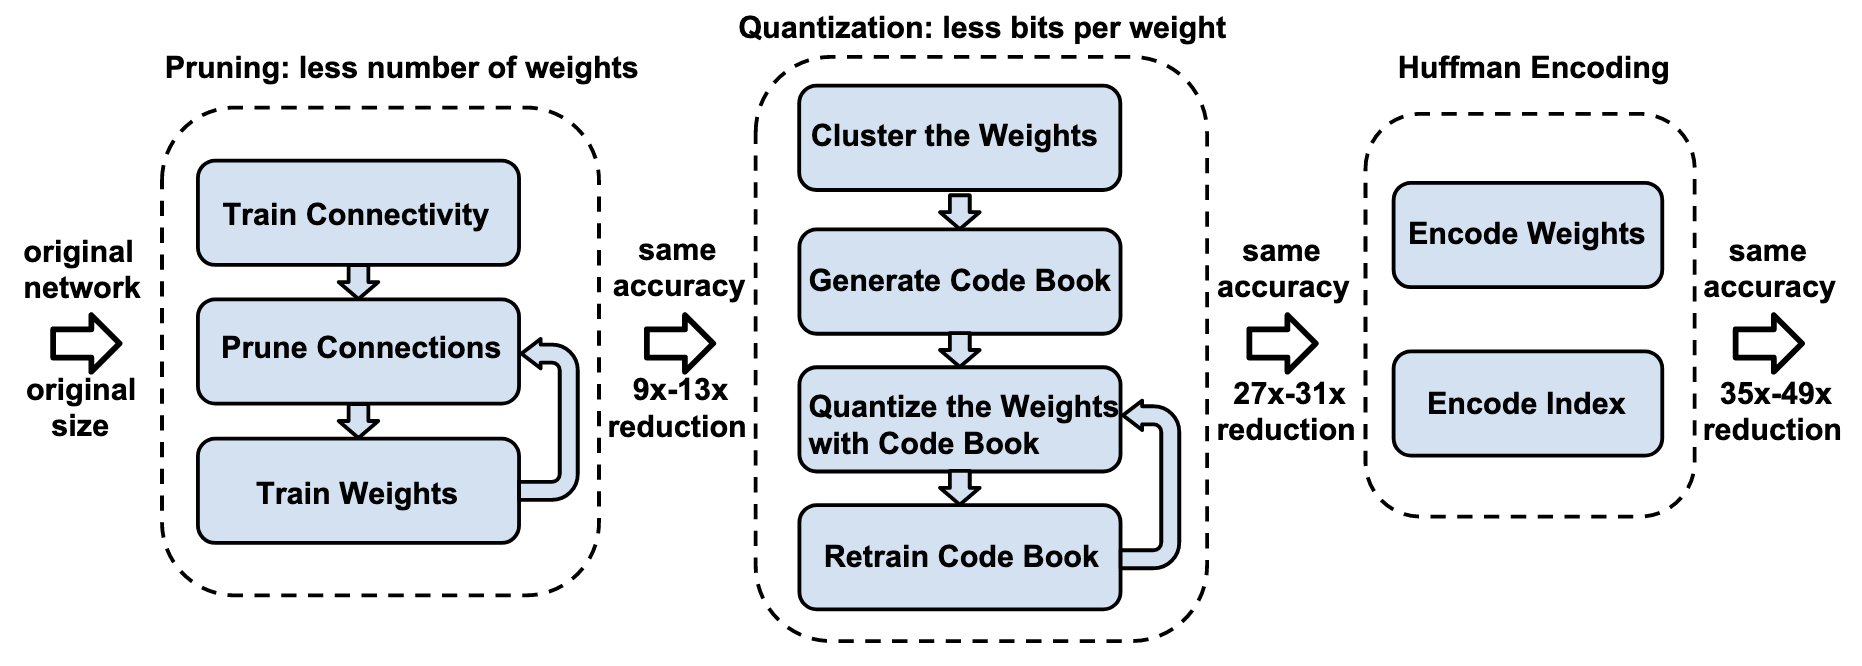
\includegraphics[width=0.9\linewidth]{images/f1_method_overview.png}
    \caption{Overview of the three stages of Deep Compression pipeline: pruning, quantization, and Huffman coding \cite{han2015deep_compression}.}
    \label{fig:method_overview}
\end{figure}

\subsection{Network Pruning}

The pruning method adopts the approach proposed in the author's previous work \ref{han2015learning}. The pruning process consists of three steps:

\begin{enumerate}
    \item Learn the connectivity via normal network training
    \item Remove the connections with small weights (below a threshold)
    \item Iteratively fine-tune/retrain the network to recover the accuracy
\end{enumerate}

The sparse matrix after pruning is stored as compressed sparse row (CSR) or compressed sparse column (CSC) format, which requires $2a+n+1$ numbers, where $a$ is the number of non-zero elements, and $n$ is the number of rows or columns.

Note that they store the index difference instead of the absolute position, and both the values and indices will be quantized later (CONVs use 8 bits, and FCs use 5 bits). If the index difference of adjacent non-zero elements exceeds the quantization range, they will use a filler zero to prevent overflow, as shown in Figure \ref{fig:filter_zero}.

\begin{figure}
    \centering
    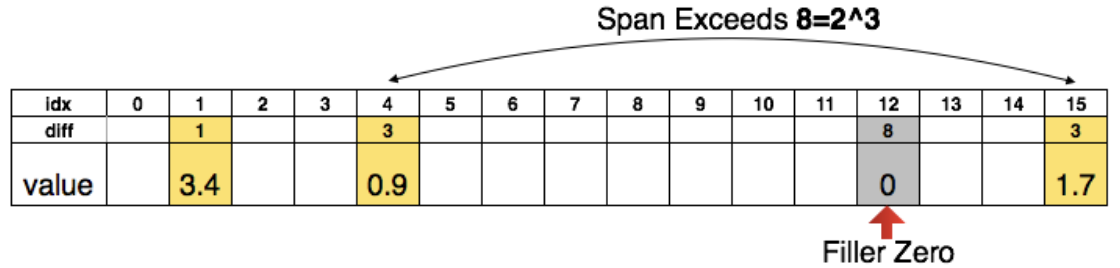
\includegraphics[width=0.8\linewidth]{images/f2_filter_zero.png}
    \caption{Representing the matrix sparsity with relative index. Padding filler zero to prevent overflow \cite{han2015deep_compression}.}
    \label{fig:filter_zero}
\end{figure}

\subsection{Trained Quantization}

As shown in Figure \ref{fig:method_overview} and \ref{fig:weight_share}, the codebook-based quantization quantization with weight sharing consists of the following steps:

\begin{enumerate}
    \item K-means clustering to find the weight value to be shared within the same cluster
    \item Generate the codebook and quantize the weights
    \item Iteratively Fine-tune the centroids in the codebook via gradient descent
\end{enumerate}

\begin{figure}
    \centering
    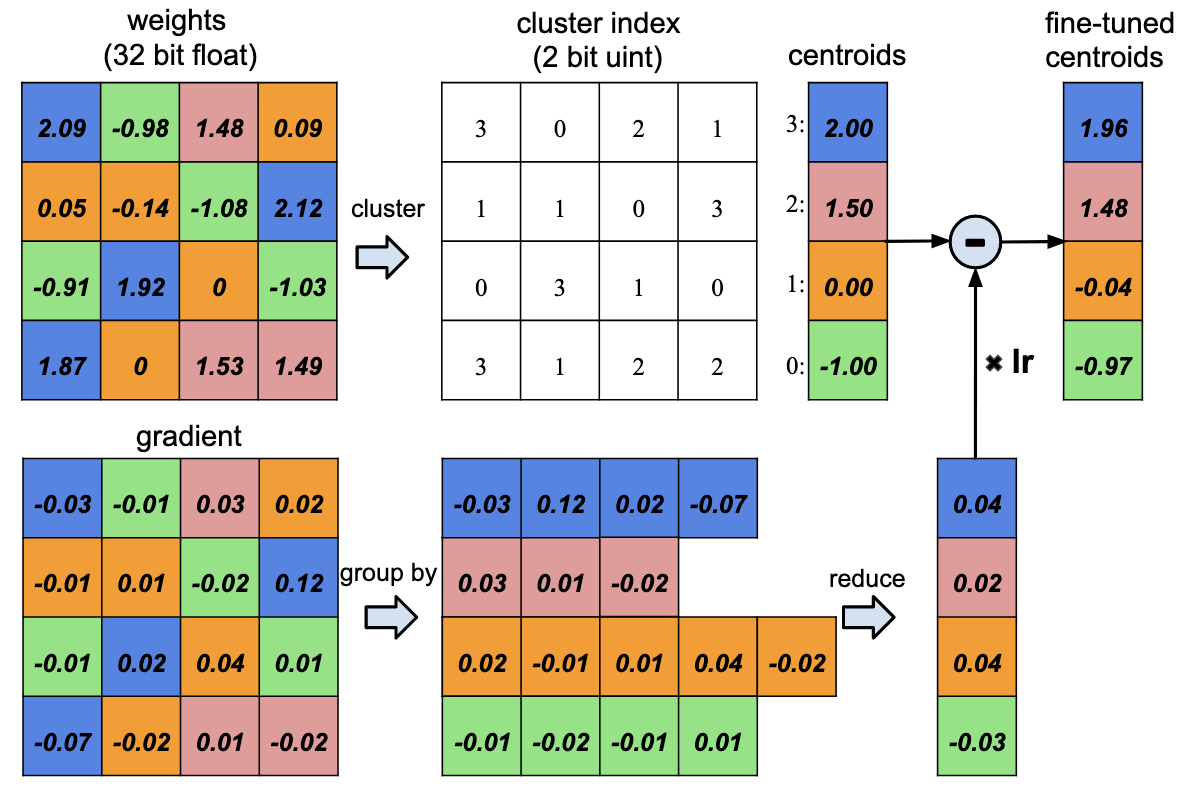
\includegraphics[width=0.8\linewidth]{images/f3_weight_share.png}
    \caption{Trained quantization process: weight sharing by scalar quantization (top) and centroid fine-tuning (bottom) \cite{han2015deep_compression}.}
    \label{fig:weight_share}
\end{figure}

Given $k$ clusters, and only $\log_2(k)$ bits are used to encode the index. For a network with n connections and each connection is represented with $b$ bits (e.g. $b=32$ for FP32), the compression rate is:

$$
r = \frac{nb}{n\log_2(k) + kb}
$$

For example, Figure \ref{fig:weight_share} shows an FC layer with $4$ inputs and $4$ outputs, so the weights has $n = 4 \times 4 = 16$ elements. The number of clusters/centroids are $k=4$, and the original floating-point numbers needs $b=32$ bits, so the compression rate is $r = \frac{16 \times 32}{16 \times 2 + 4 \times 32} = 3.2$.

% They use k-means clustering algorithm to find the weight value to be shared within the same cluster. They partition $n$ original weights $W = \{ w_1, w_2, ..., w_n \}$ into $k$ clusters $C = \{ c_1, c_2, ..., c_k \}, n>>k$. The loss function is the within-cluster sum of squares (WCSS):

% $$
% \text{arg}\min_C \sum_{i=1}^{k} \sum_{w_j \in c_i} || w_j - c_i ||^2
% $$

% $$
% \frac{\partial L}{\partial C_k} = \sum_{i,j} \frac{\partial L}{\partial W_{ij}} \frac{\partial W_{ij}}{\partial C_k} = \sum{i,j} \frac{\partial L}{\partial W_{ij}} \mathbf{1}(I_{ij} = k)
% $$

\subsection{Huffman Coding}

Huffman coding is a lossless data compression technique that assigns variable-length codes to the inputs based on their frequency of occurrence. The more frequent the input, the shorter the code. Figure \ref{fig:weight_dist} shows the distribution of weight (left) and sparse matrix index (right) of the last FC layer in AlexNet, which have large variance in their frequency, and it is therefore suitable for Huffman coding.

\begin{figure}[h]
    \centering
    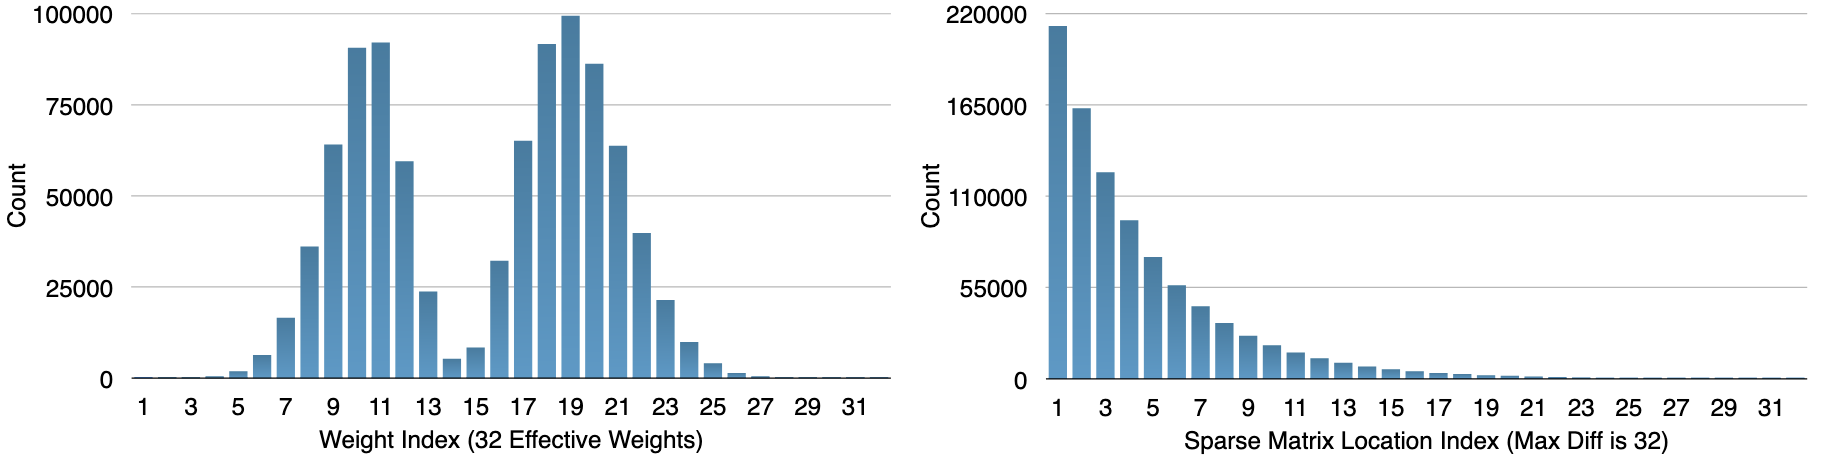
\includegraphics[width=0.8\linewidth]{images/f5_weight_dist.png}
    \caption{Distribution of weight (left) and sparse matrix index (right) \cite{han2015deep_compression}.}
    \label{fig:weight_dist}
\end{figure}

\section{Experiment and Evaluation}

\subsection{Image Classification Tasks}

\begin{figure}
    \centering
    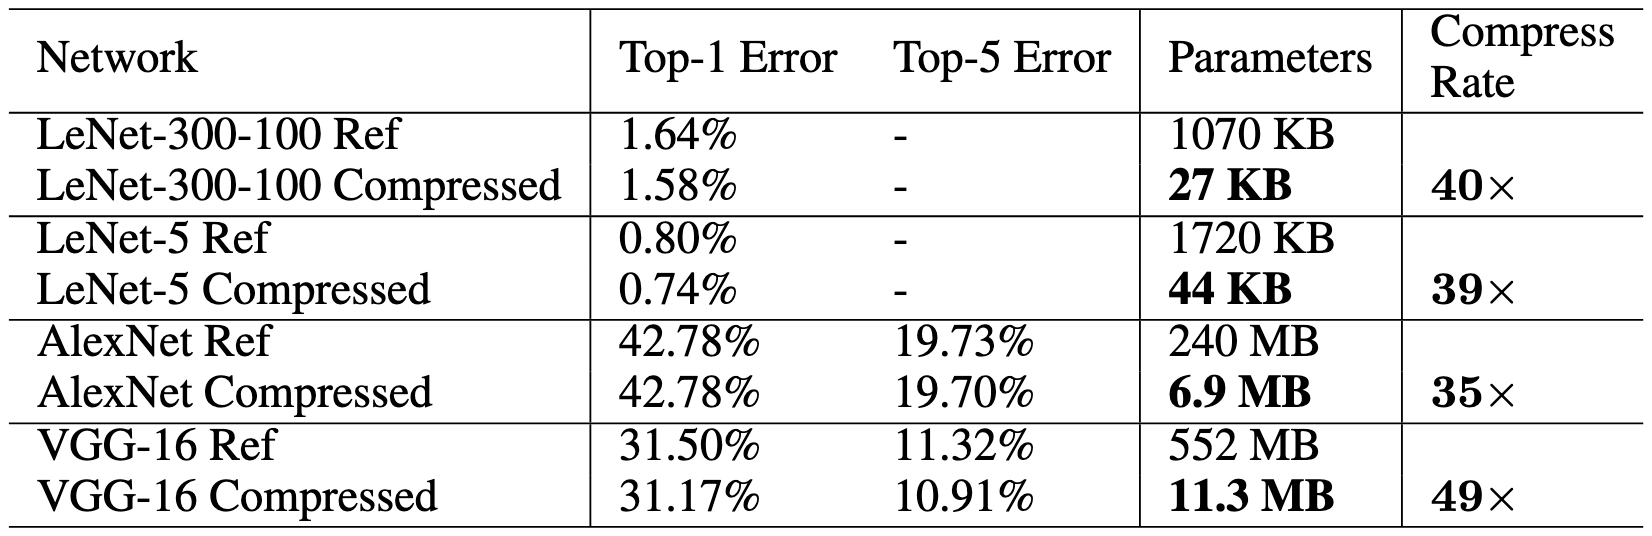
\includegraphics[width=0.9\linewidth]{images/t1_result.png}
    \caption{The top-1 and top-5 errors and compression rate before/after applying the proposed compression method.}
    \label{fig:result}
\end{figure}

\begin{figure}
    \centering
    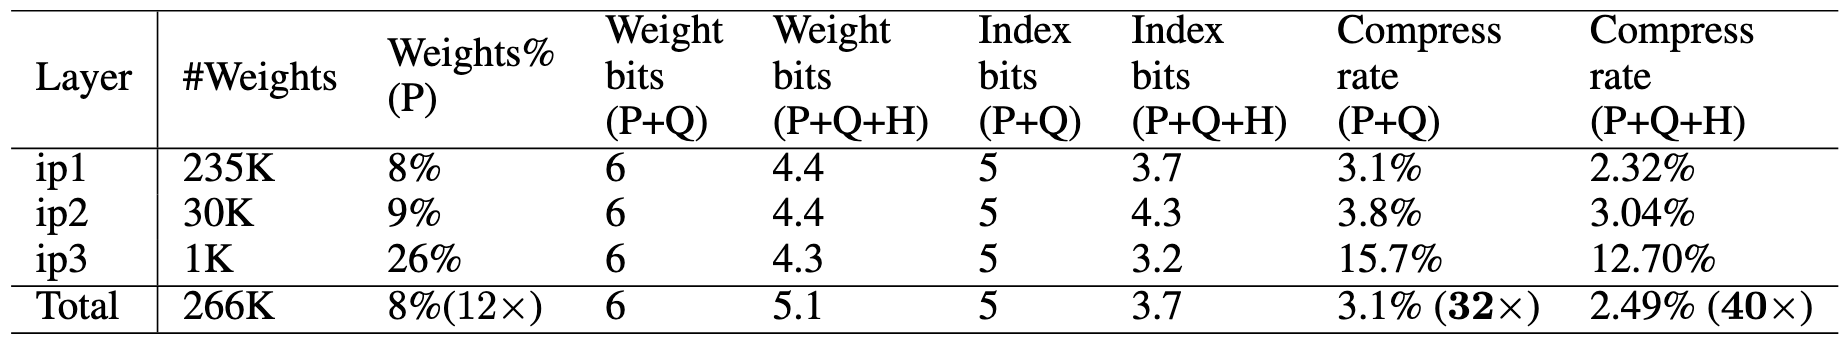
\includegraphics[width=0.9\linewidth]{images/t2_lenet_300_100.png}
    \caption{LeNet-300-100 on MNIST.}
    \label{fig:lenet_300_100}
\end{figure}

\begin{figure}
    \centering
    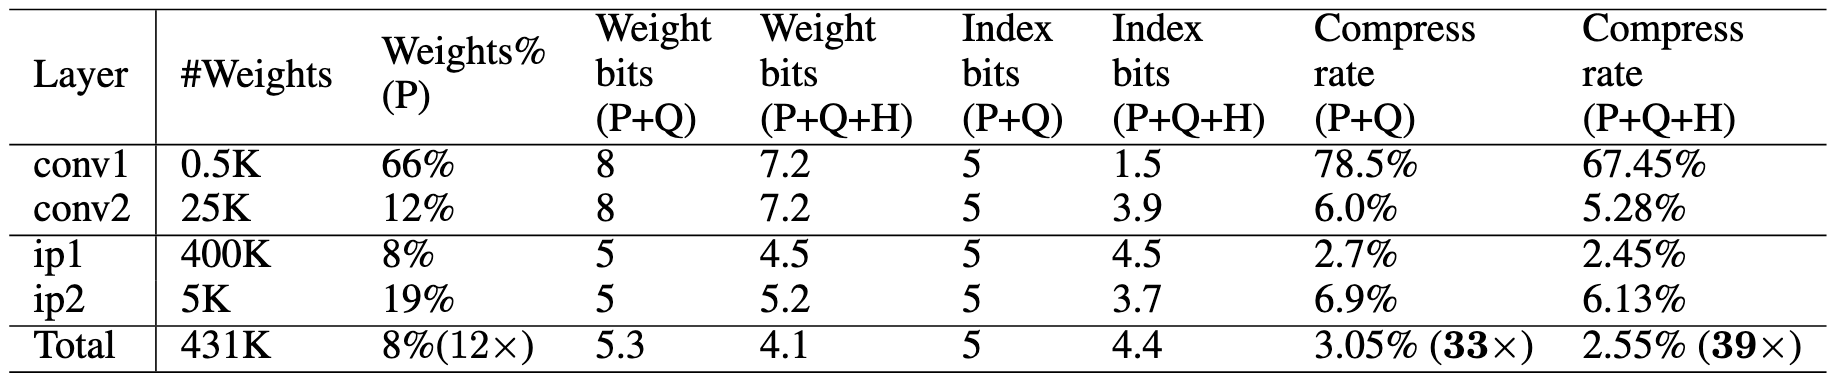
\includegraphics[width=0.9\linewidth]{images/t3_lenet5.png}
    \caption{LeNet-5 on MNIST.}
    \label{fig:lenet5}
\end{figure}

\begin{figure}
    \centering
    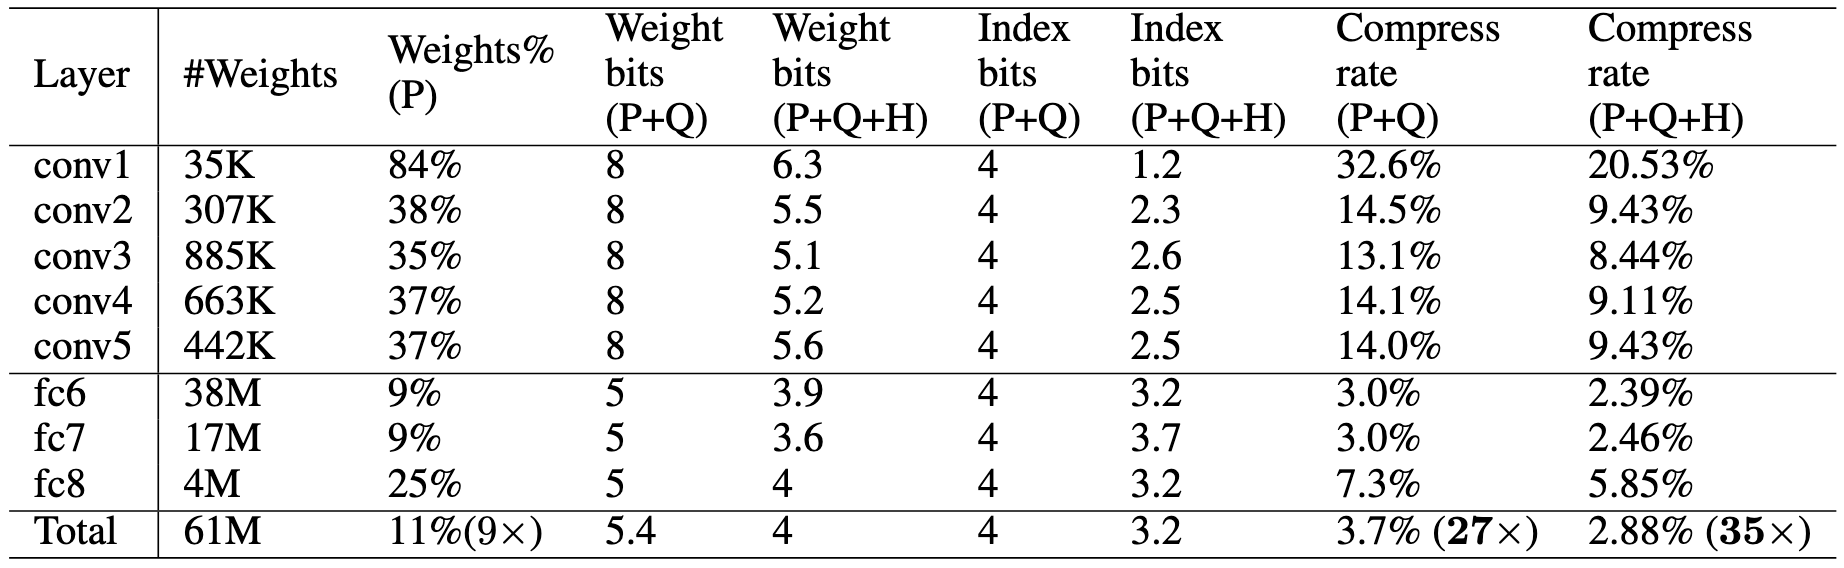
\includegraphics[width=0.9\linewidth]{images/t4_alexnet.png}
    \caption{AlexNet on ImageNet.}
    \label{fig:alexnet}
\end{figure}

\begin{figure}
    \centering
    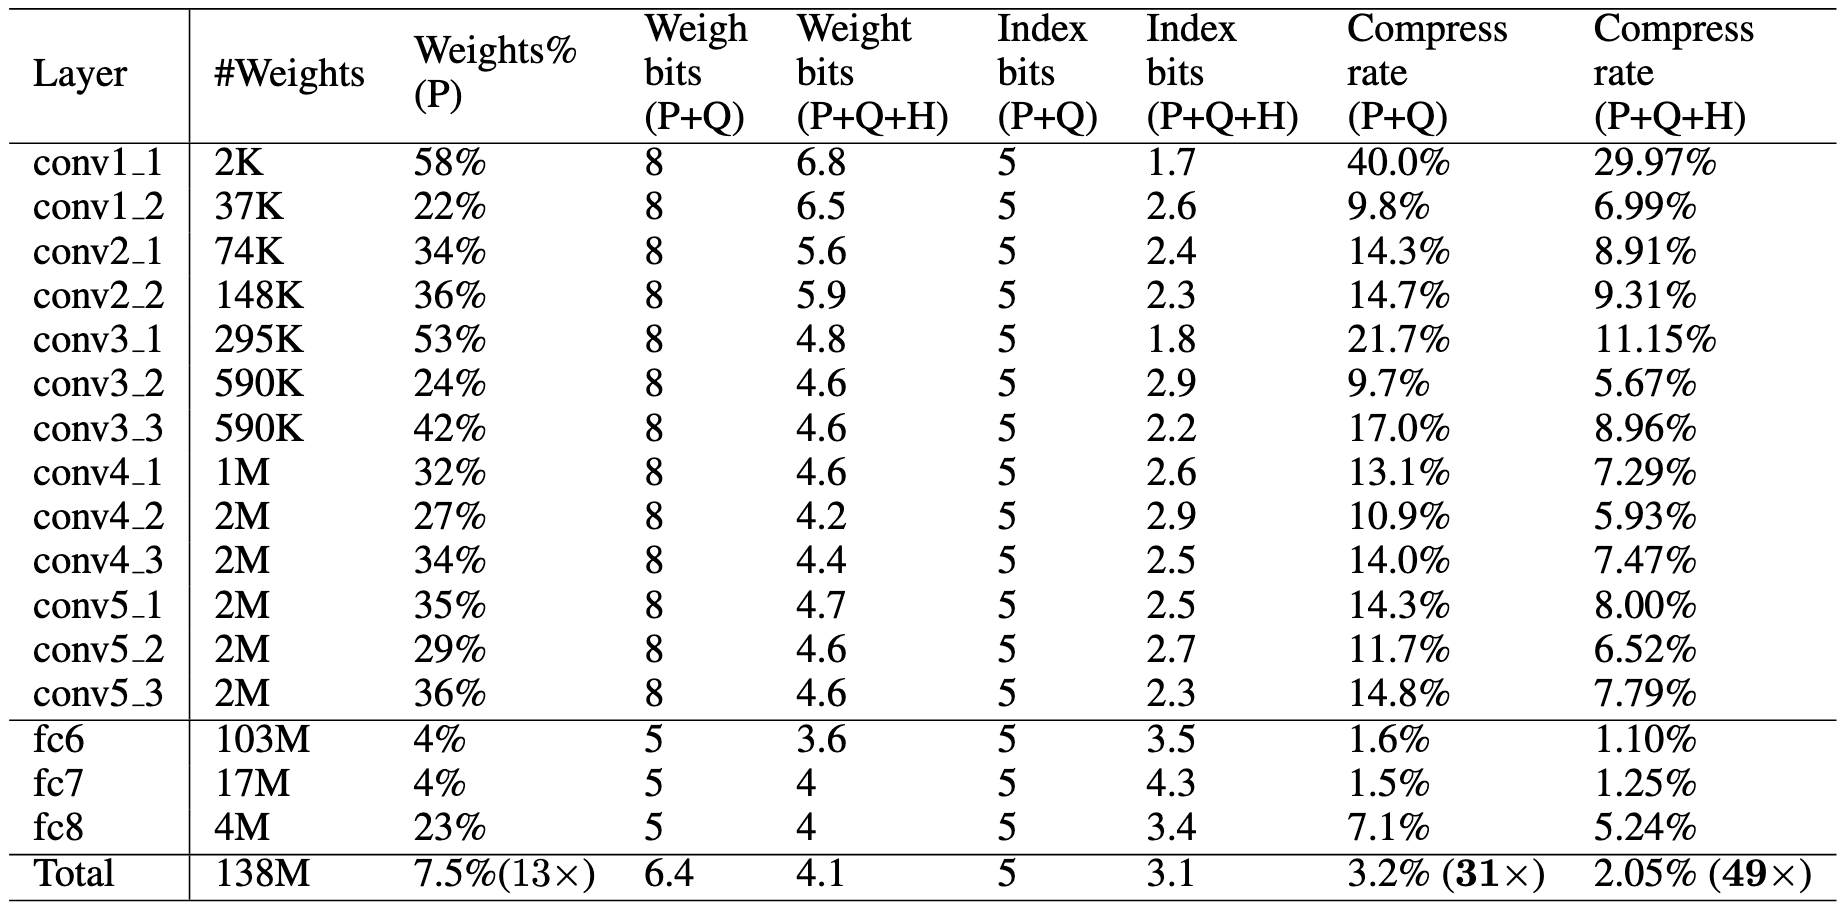
\includegraphics[width=0.9\linewidth]{images/t5_vgg16.png}
    \caption{VGG-16 on ImageNet.}
    \label{fig:vgg16}
\end{figure}

They evaluate the proposed method on the following image classification tasks, and the results are shown in Table \ref{fig:result}. The compression statistics are shown in Table \ref{fig:lenet_300_100}, \ref{fig:lenet5}, \ref{fig:alexnet}, and \ref{fig:vgg16}.

\begin{enumerate}
    \item LeNet-300-100 on MNIST (Figure \ref{fig:lenet_300_100})
    \item LeNet-5 on MNIST (Figure \ref{fig:lenet5})
    \item AlexNet on ImageNet (Figure \ref{fig:alexnet})
    \item VGG-15 on ImageNet (Figure \ref{fig:vgg16})
\end{enumerate}

\subsection{Pruning and Quantization Working Together}

\begin{figure}
    \centering
    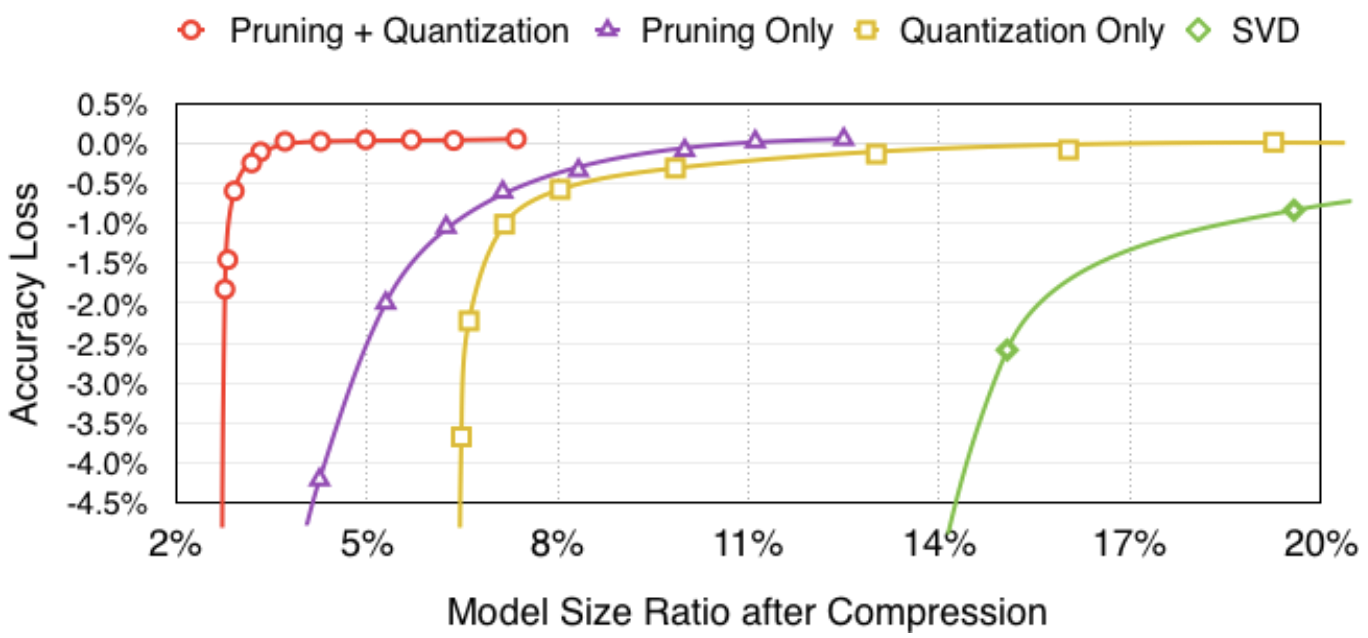
\includegraphics[width=0.7\linewidth]{images/f6_prune_quant.png}
    \caption{Accuracy v.s. compression rate under different compression methods. Pruning + quantization works the best.}
    \label{fig:prune_quant}
\end{figure}

\begin{figure}
    \centering
    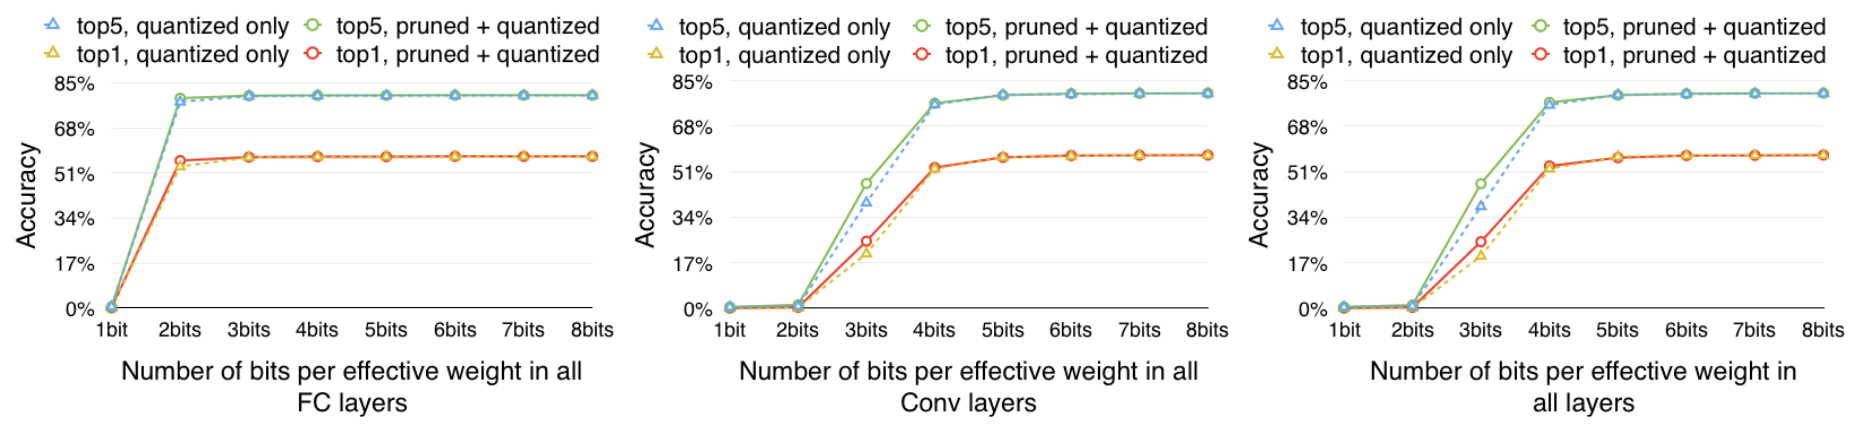
\includegraphics[width=0.9\linewidth]{images/f7_acc_drop.png}
    \caption{Accuracy v.s. compression rate under different compression methods. Pruning + quantization + Huffman coding works the best.}
    \label{fig:acc_drop}
\end{figure}

Figure \ref{fig:prune_quant} shows pruning combined with quantization (the leftest read line) works the best. Even being compressed to 3\% of the original size, there is no loss of accuracy.

Figure \ref{fig:acc_drop} shows the accuracy between quantization only and pruning + quantization under different number of bits. For both CONVs and FCs, pruning works well with quantization.

\subsection{Centroid Initialization}

This paper have tried three different methods for centroids initialization (Figure \ref{fig:centroid_init}):

\begin{enumerate}
    \item Random initialization: randomly select $k$ observations from the dataset
    \item Density-based initialization: linearly spaces the centroids of the weights in the y-axis, then find the corresponding x-axis value.
    \item Linear initialization: linearly spaces the centroids of the weights between [min, max] in the x-axis
\end{enumerate}

\begin{figure}
    \centering
    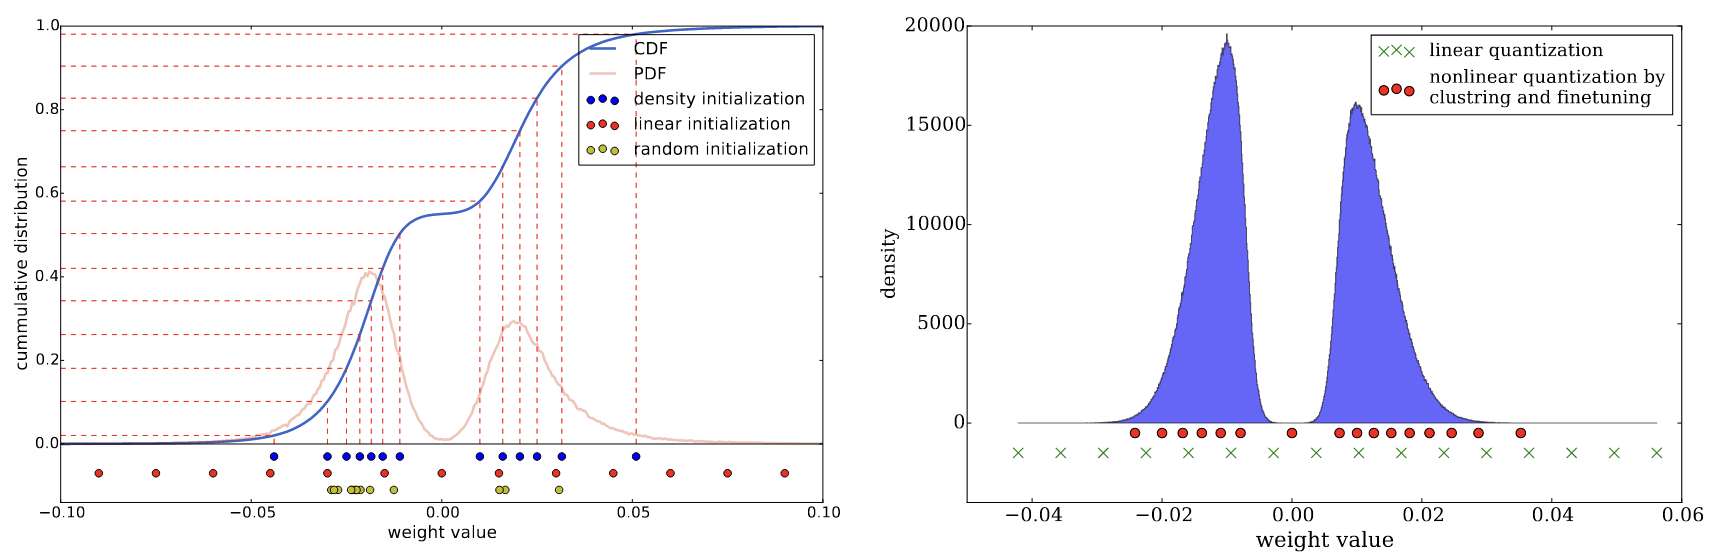
\includegraphics[width=0.8\linewidth]{images/f4_centroid_init.png}
    \caption{Left: Three different methods for centroids initialization. Right: Distribution of weights (blue) and distribution of codebook before (green cross) and after fine-tuning (red dot) \cite{han2015deep_compression}.}
    \label{fig:centroid_init}
\end{figure}

Figure \ref{fig:centroid_init_eval} compares the accuracy of the three different initialization methods. Linear initialization outperforms the other two methods in all cases except at 3 bits.

\begin{figure}
    \centering
    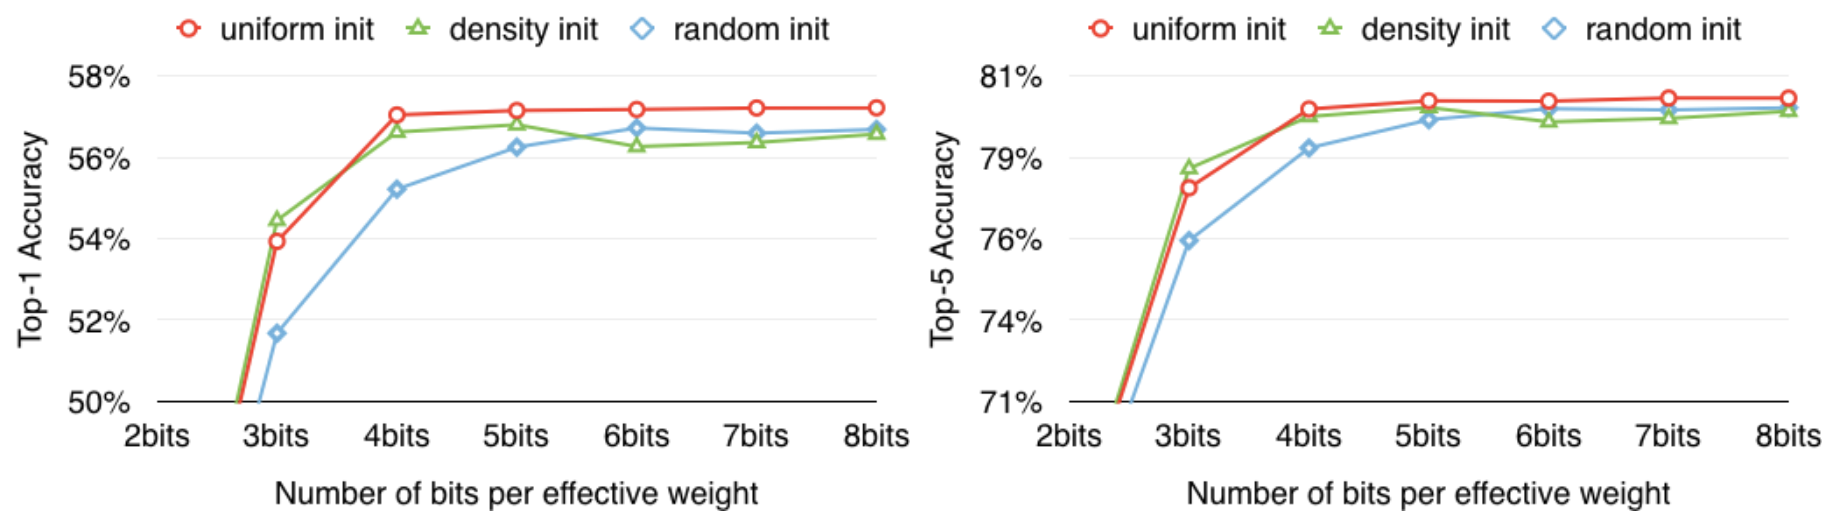
\includegraphics[width=0.9\linewidth]{images/f8_centroid_init_eval.png}
    \caption{Three different methods for centroids initialization.}
    \label{fig:centroid_init_eval}
\end{figure}

\subsection{Speedup and Energy Efficiency}

Figure \ref{fig:prune_speedup} illustrates the speedup of pruning on different hardware. When batch size is 1, the pruned network obtains 3x to 4x speedup over the dense network due to the smaller memory footprint and less data transferring overhead.

Figure \ref{fig:prune_energy} illustrates the energy efficiency of pruning on different hardware. When batch size is 1, the pruned network comsumes 3x to 7x less energy over the dense network.

\begin{figure}
    \centering
    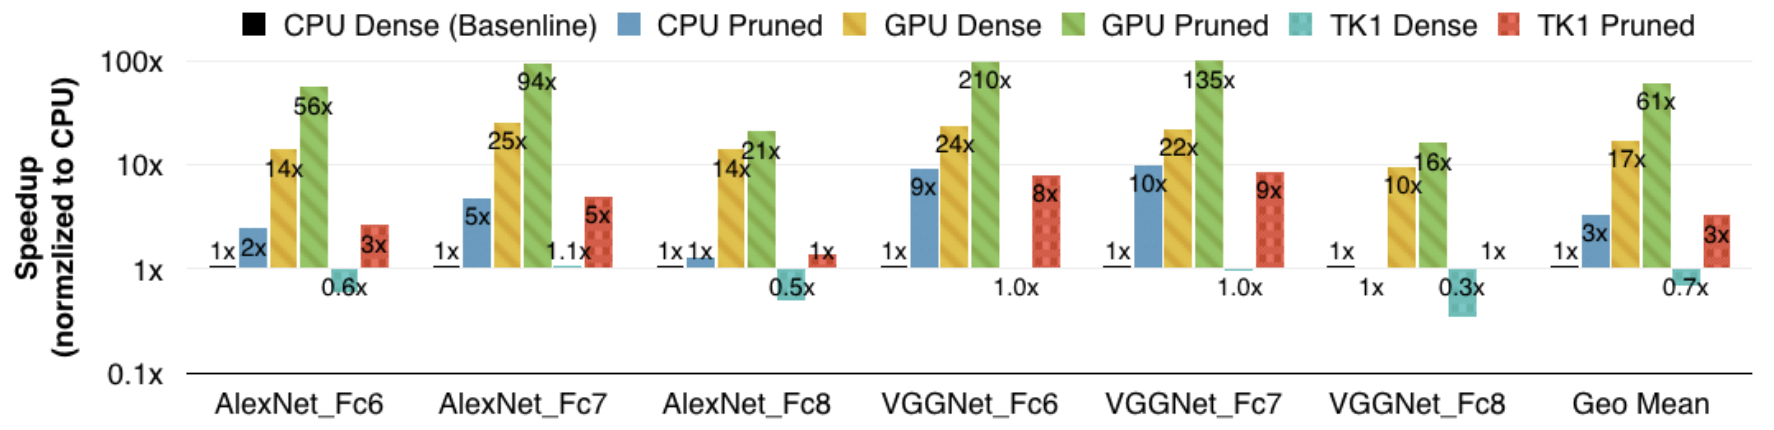
\includegraphics[width=0.9\linewidth]{images/f9_prune_speedup.png}
    \caption{Speedup comparison on different hardware.}
    \label{fig:prune_speedup}
\end{figure}

\begin{figure}
    \centering
    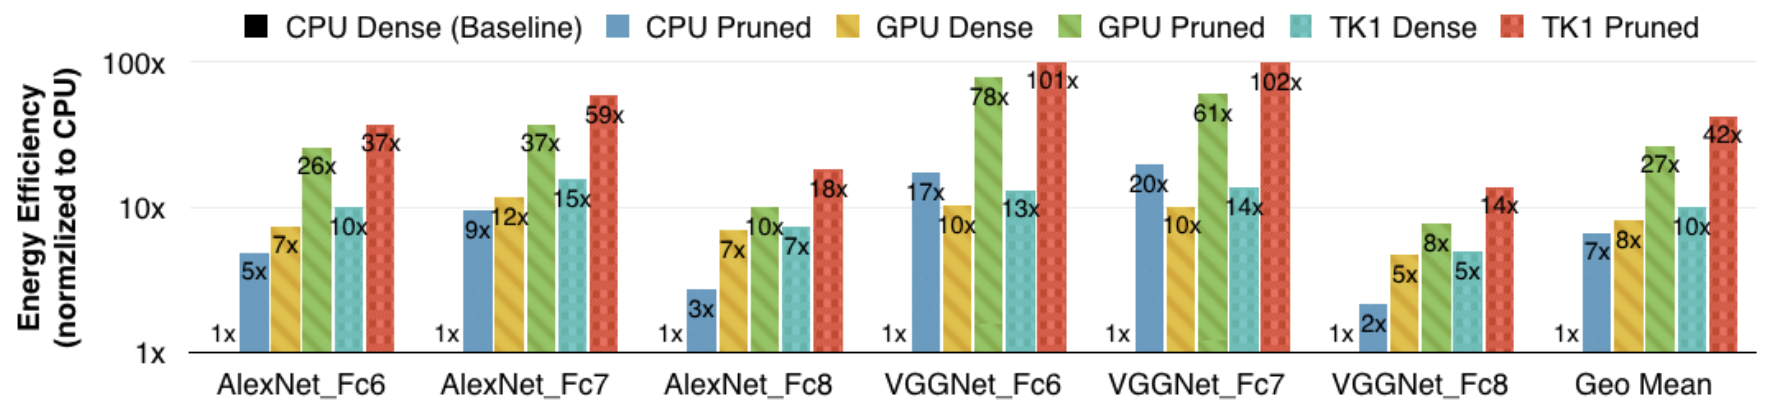
\includegraphics[width=0.9\linewidth]{images/f10_prune_energy.png}
    \caption{Energy efficiency comparison on different hardware.}
    \label{fig:prune_energy}
\end{figure}

\subsection{Ratio of Weights, Index, and Codebook}

As Figure \ref{fig:storage_ratio} shows, the storage of  weights and the sparse indexes are roughly half and half respectively since on average they are encoded with 5 bits. The overhead of codebook is very small and often negligible.

\begin{figure}
    \centering
    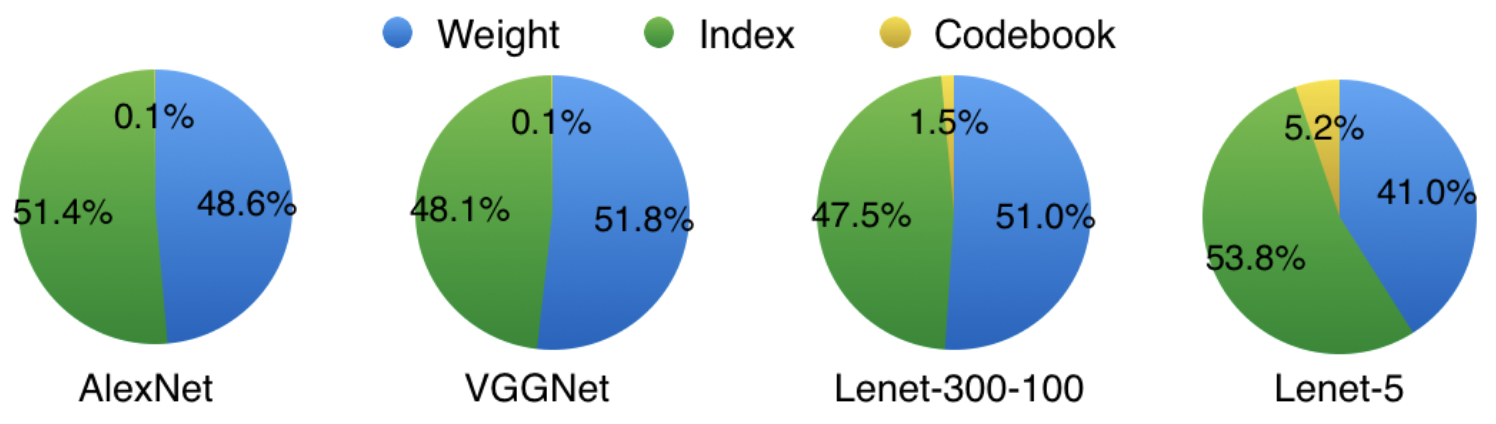
\includegraphics[width=0.7\linewidth]{images/f11_storage_ratio.png}
    \caption{The storage ratio of weights, index, and codebook in the compressed model.}
    \label{fig:storage_ratio}
\end{figure}

\section{Analysis}

This paper has the following advantages and disadvantages:

\subsection{Advantages}

\begin{itemize}
    \item \textbf{Proposed a systematic compression framework}\\
    Combines pruning, quantization, and encoding into a complete compression framework, forming an end-to-end process from model training to deployment, providing a clear methodology for model compression.

    \item \textbf{Multi-stage compression strategy}\\
    Sequentially applies pruning to reduce redundant connections, quantization to lower bit width, and Huffman coding to further compress storage requirements. Each step has a clear technical goal and complements the others.
    This strategy achieves a compression ratio of up to 35–49×, demonstrating significant effectiveness.

    \item \textbf{Practicality of pruning methods}\\
    Uses importance-based weight pruning to effectively remove redundant parameters with minimal impact on model performance, significantly reducing model size.
    Fine-tuning the pruned model can restore its original performance.

    \item \textbf{Innovative quantization techniques}\\
    Introduces weight sharing and quantization, significantly reducing the number of bits needed by representing weights using cluster centers and index-based storage.
    Compared to traditional quantization techniques, this approach maintains model accuracy by leveraging learned cluster centers.

    \item \textbf{Comprehensive theoretical and experimental validation}\\
    Provides experimental results on multiple models (e.g., AlexNet and VGG-16), demonstrating the method's effectiveness across various deep learning applications.
    Quantitative analysis of the trade-off between compression ratio and model performance showcases its ability to achieve efficient compression while maintaining accuracy.

    \item \textbf{Strong generality}\\
    The framework is not limited to specific neural network architectures or application scenarios, exhibiting strong generality and applicability to various CNN models.

    \item \textbf{Reduces deployment cost}\\
    By compressing the model, it significantly reduces storage and transmission costs, facilitating the deployment of deep learning models on resource-constrained devices, such as mobile and embedded systems.

    \item \textbf{Decreases energy consumption and computation cost}\\
    Pruning and quantization not only reduce model size but also decrease the number of multiplication operations during inference, effectively lowering energy consumption and inference latency.

    \item \textbf{Compatibility with existing techniques}\\
    Techniques like Huffman coding can seamlessly integrate with existing compression methods, further improving compression efficiency with minimal impact on the training process.
\end{itemize}

\subsection{Disadvantages}

\begin{itemize}
    \item \textbf{Weight sharing via k-means limitations}\\
    The k-means-based weight sharing approach forces unrelated weight elements to update together, as similar values are grouped, which may negatively impact training.

    \item \textbf{Quantization using codebooks}\\
    Although codebook quantization replaces most floating-point operations with integer operations, floating-point computations are still required during both fine-tuning and inference.

    \item \textbf{Unstructured pruning's hardware unfriendly nature}\\
    The unstructured pruning approach is less hardware-friendly. The CSR or CSC compressed encoding used is not supported by all hardware. Software-based transformations (e.g., special kernel libraries) introduce additional overhead, and decompressing before computation negates the benefits of compression, such as reduced memory footprint, data movement, and off-chip DRAM accesses.

    \item \textbf{Huffman coding's inference overhead}\\
    Huffman coding introduces additional decoding operations during inference, potentially increasing computation overhead on general-purpose hardware like CPUs or GPUs. Whether the reduced memory access overhead compensates for the encoding/decoding overhead requires further analysis and comparison with other compression methods, such as weight decomposition or knowledge distillation.

    \item \textbf{Lack of support for ultra-low precision}\\
    The paper primarily explores higher-bit quantization (8-bit for CONVs and 5-bit for FCs), but does not address challenges of ultra-low precision. Modern Transformer models often adopt more aggressive low-precision formats (e.g., INT4 or lower) for efficient deployment.

    \item \textbf{Insufficient hardware-specific optimizations}\\
    The compressed models (via quantization and pruning) may not fully leverage the theoretical compression benefits on specific hardware (e.g., GPUs, TPUs). Hardware not optimized for sparse matrix operations offers limited performance gains.

    \item \textbf{Lack of structured pruning}\\
    Structured pruning (e.g., removing entire rows or blocks of parameters) is more suited for hardware acceleration. This paper focuses on unstructured pruning, which is less hardware-friendly.

    \item \textbf{Limited evaluation on modern architectures}\\
    At the time, architectures like ResNet, MobileNet, EfficientNet, and Transformer were not yet developed. The applicability of the proposed methods to these newer architectures requires further exploration.
\end{itemize}

\section{Future Directions}

\begin{itemize}
    \item \textbf{Huffman Coding and Precision Optimization}: Huffman coding encodes quantized numbers based on their frequency, using fewer bits for common values and more bits for rare values. In current Transformer families, outliers often appear in activations, with most elements having similar magnitudes. This approach is similar to mixed precision quantization. A potential optimization could involve combining these techniques: applying Huffman coding on mixed-precision quantized numbers and accelerating through hardware implementation.

    \item \textbf{Limitations of K-means Weight Sharing}: The paper's k-means weight sharing approach forces unrelated weight elements to update together, despite similar values not necessarily indicating synchronous updates. A better approach would involve considering gradient dynamics during clustering and redesigning the WSCC loss function to more accurately capture weight element relationships.

    \item \textbf{Structured Pruning}: Extend pruning from unstructured to structured approaches, targeting attention heads, Transformer layers, or entire modules to better leverage hardware characteristics like sparse matrix multiplication acceleration.

    \item \textbf{Quantization Optimization}: Support ultra-low precision quantization (e.g., INT4 or binarization) combined with mixed-precision techniques, preserving precision for critical components while reducing bit width for others.

    \item \textbf{Sparsity Optimization and Dynamic Sparsity}: Leverage the inherent sparsity in modern LLM attention mechanisms through learned sparsity methods like sparse attention and long-range sparse mechanisms to further reduce computational complexity.

    \item \textbf{Multimodal Architecture-Specific Compression}: Design specialized compression techniques for different modalities in multimodal models, such as CNN-inspired methods for image modalities and language knowledge distillation for text modalities.

    \item \textbf{Combining Distillation and Compression}: Utilize knowledge distillation and deep compression as complementary techniques, transferring knowledge from large Transformer models to smaller, compressed models while integrating pruning and quantization.

    \item \textbf{End-to-End Optimization}: Develop end-to-end training processes specifically for compression techniques, rather than applying them post-training, to minimize performance impact from pruning and quantization.
\end{itemize}

%%%%%%%%%%%%%%%%%%%%%%%%%%%%%%%%%%%%%%%%%%%%%%%%%%%%%%%%%%%%

% \pagebreak
% \printbibliography
\printbibliography  % Print the bibliography
\end{document}
